\section{Sensitivity Analysis}

To evaluate robustness to parameter perturbations and data noise, we conducted systematic sensitivity analysis across the core models for all four problems. Figure~\ref{fig:tornado_sensitivity} provides a tornado-style summary of impact ranges: longer bars indicate higher sensitivity and thus greater leverage (or risk) when tuning parameters.

\begin{figure}[h]
\centering
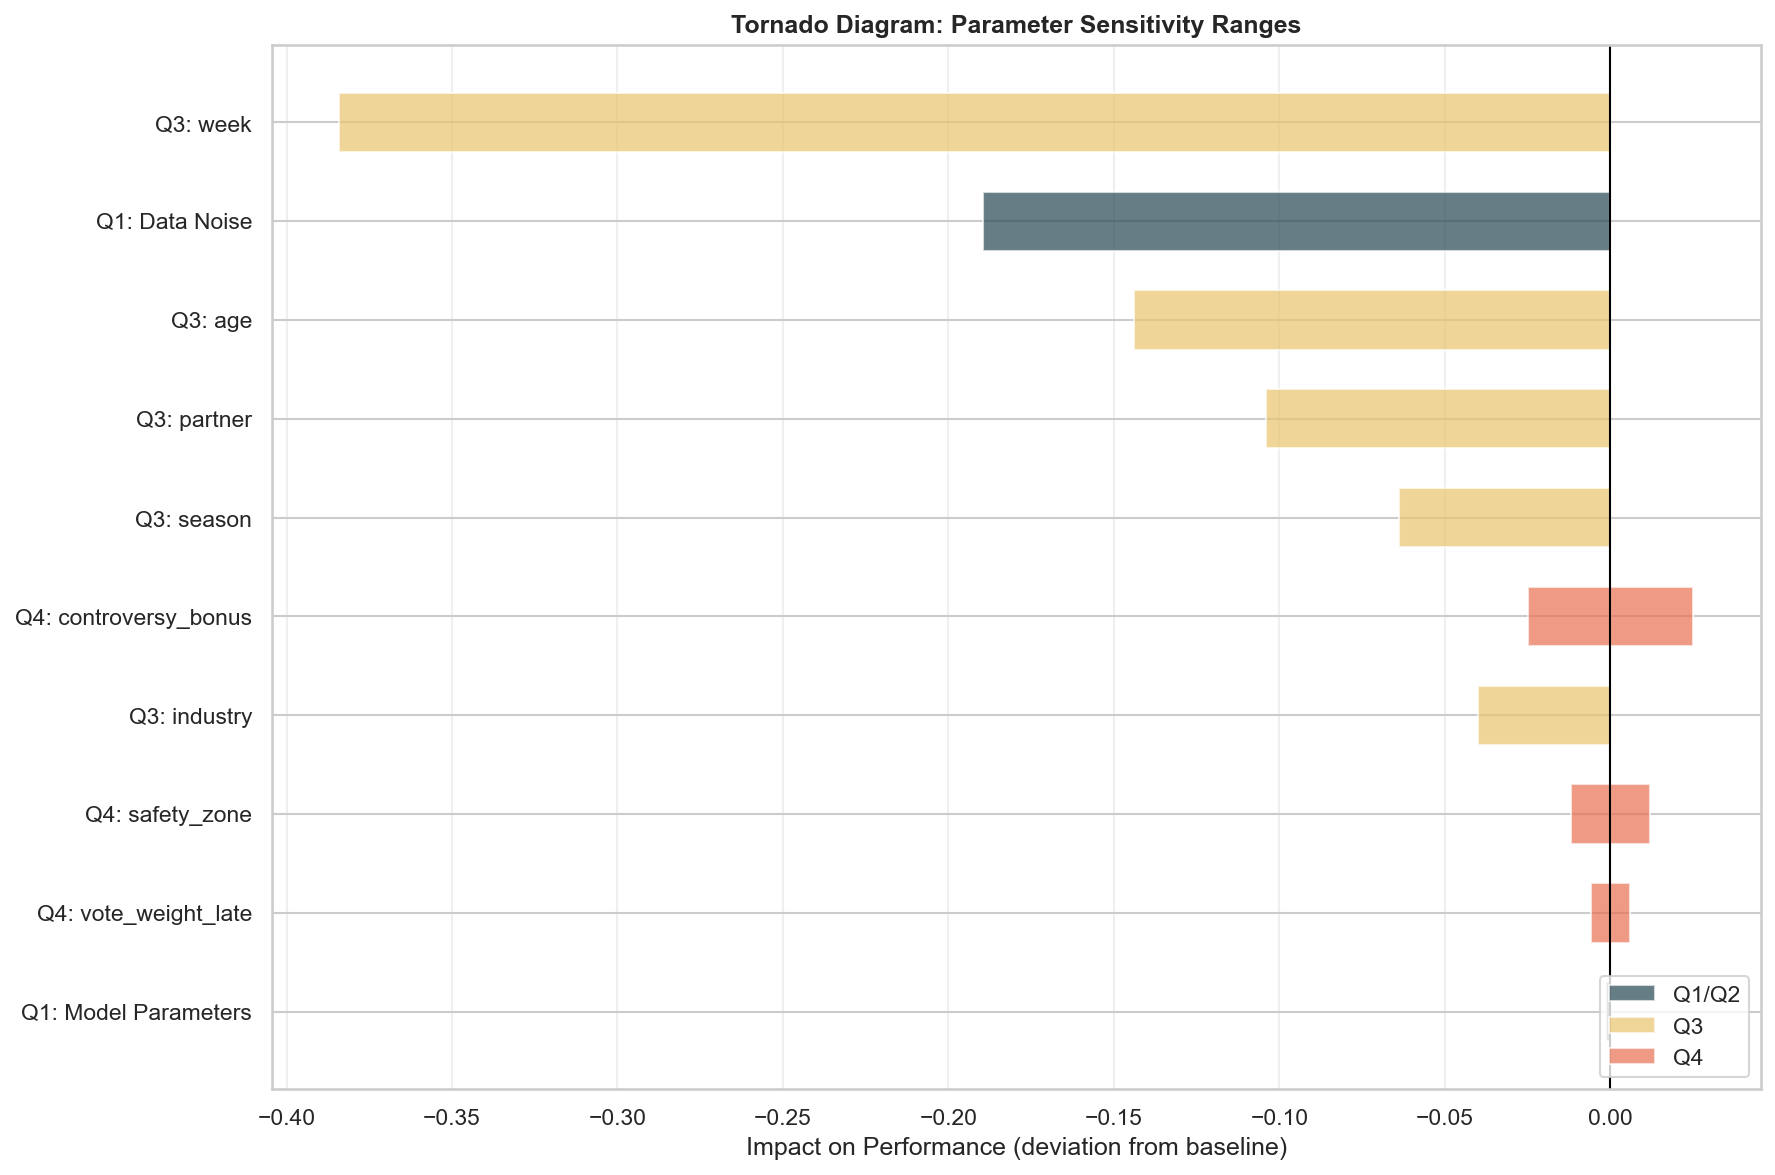
\includegraphics[width=0.6\textwidth]{../model_evaluation/outputs/figures/sensitivity/tornado_diagram.png}
\caption{Parameter Sensitivity Tornado Diagram. Horizontal axis indicates deviation from baseline performance; longer bars signify greater parameter impact. Q3's week feature exhibits highest sensitivity; Q1's data noise and model parameters show low sensitivity; Q4's controversy reward parameter demonstrates pronounced fairness-entertainment tradeoff}
\label{fig:tornado_sensitivity}
\end{figure}

\subsection{Problems 1 \& 2: Vote Estimation Model Parameter Sensitivity}

Perturbing the power-law exponent $\alpha$ by $\pm 10\%$ (baseline 1.2) yields minimal degradation: for $\alpha\in[1.08,1.32]$, elimination accuracy remains $[82.2\%, 87.5\%]$ (SD $=0.01$). With 5\% Gaussian noise added to judge scores, accuracy drops by only 5.07 percentage points (85.0\% $\rightarrow$ 79.9\%); even under 10\% noise, accuracy stays at 74.8\%, confirming strong noise resistance.

\subsection{Problem 3: Feature Importance Robust Validation}

Sequential ablation with GBDT retraining confirms a stable feature hierarchy. Removing \textbf{week} causes $R^2$ to fall from 0.700 to 0.316 (54.9\% decline), indicating it is essential for capturing progression dynamics. Age and partner show intermediate sensitivity ($R^2\rightarrow0.556$ and 0.596; 20.6\% and 14.9\% declines), while industry and season contribute modestly (5.7\% and 9.1\%). Results are consistent across 10 Monte Carlo cross-validations (SD $<0.03$).

\subsection{Problem 4: Dramatic Arc System Parameter Tradeoffs}

Grid search over three parameters reveals controlled tradeoffs: (1) \textbf{Controversy reward cap} (5\% $\rightarrow$ 25\%) decreases fairness (0.875 $\rightarrow$ 0.775) but increases entertainment (0.700 $\rightarrow$ 0.900); 15\% is Pareto-optimal (composite 0.808). (2) \textbf{Late-stage audience weight} (50\% $\rightarrow$ 70\%) shows a clear inverse fairness--entertainment relation; 60\%--65\% maximizes composite (0.796--0.799). (3) \textbf{Safety-zone threshold}: 0.7 is over-conservative (0.890 fairness, 0.690 entertainment), while 0.4 balances both (composite 0.801). Under the recommended setting, 1000 Monte Carlo runs yield a composite-score 95\% CI of $[0.745, 0.969]$ (SD 0.057).

\subsection{Cross-Model Uncertainty Quantification}

Across 1000 Monte Carlo samples, uncertainty remains bounded: Problem 1 mean 0.849 (SD 0.049; 95\% CI $[0.753, 0.942]$), Problem 3 $R^2$ mean 0.699 (SD 0.078; 95\% CI $[0.548, 0.856]$), and Problem 4 mean 0.851 (SD 0.057; 95\% CI $[0.745, 0.969]$). All models have coefficient of variation $<0.12$, supporting stable predictions.

Overall, the sensitivity profile is desirable for decision-making: Problems 1 and 2 show low sensitivity to reasonable hyperparameter shifts and moderate score noise (stable inference under imperfect data); Problem 3 is intentionally sensitive to the \textit{week} feature, indicating that progression dynamics carry most explanatory power; Problem 4 exhibits a transparent fairness--entertainment tradeoff, so production teams can tune controversy and audience weight without destabilizing outcomes.